\documentclass[12pt, twoside]{article}
\usepackage[letterpaper, margin=1in, headsep=0.5in]{geometry}
\usepackage[english]{babel}
\usepackage[utf8]{inputenc}
\usepackage{amsmath}
\usepackage{amsfonts}
\usepackage{amssymb}
\usepackage{tikz}
\usetikzlibrary{quotes, angles}
\usepackage{graphicx}
\usepackage{enumitem}
\usepackage{multicol}

\newif\ifmeta
\metatrue %print standards and topics tags

\title{Regents Geometry}
\author{Chris Huson}
\date{November 2021}

\usepackage{fancyhdr}
\pagestyle{fancy}
\fancyhf{}
\renewcommand{\headrulewidth}{0pt} % disable the underline of the header
\raggedbottom


\fancyhead[LE]{\thepage}
\fancyhead[RO]{\thepage \\ Name: \hspace{4cm} \,\\}
\fancyhead[LO]{BECA / Dr. Huson / Geometry 04 Analytic Geometry}

\begin{document}

\subsubsection*{4.12 Do Now Quiz: Linear equations \hfill CCSS.HSG.GPE.B.5}
\begin{enumerate}
\item The line $l$ is graphed at right.
\begin{multicols}{2}
\begin{enumerate}
  \item Write down the line's slope.\\ $m=$
  \vspace{0.5cm}
  \item Write down it's $y$-intercept.\\ $b=$
  \vspace{0.5cm}
  \item Write down the equation of the line.
  \vspace{1.5cm}
  \item Draw a line parallel to $l$ through point $P$. (use a straight edge for full credit)
\end{enumerate} \vspace{.5cm}
  \begin{center} 
  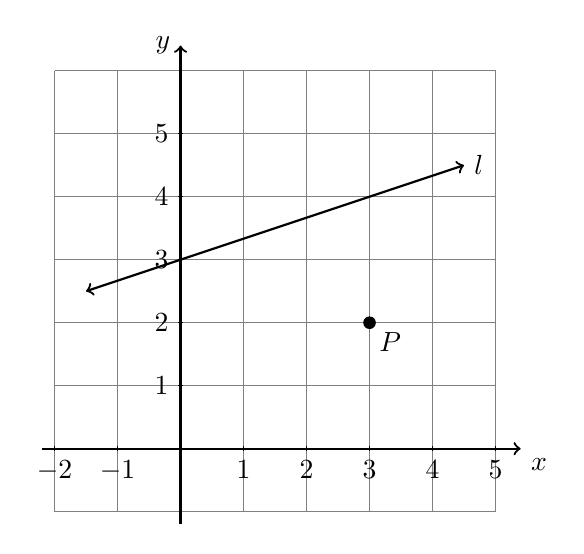
\begin{tikzpicture}[scale=0.8]
    \draw [help lines] (-2,-1) grid (5,6);
    \draw [thick, ->] (-2.2,0) -- (5.4,0) node [below right] {$x$};
    \draw [thick, ->] (0,-1.2)--(0,6.4) node [left] {$y$};
    \foreach \x in {-2,-1,1,2,...,5} \draw (\x cm,1pt) -- (\x cm,-1pt) node[anchor=north] {$\x$};
    \foreach \y in {1, 2, 3, 4, 5} \draw (1pt,\y cm) -- (-1pt,\y cm) node[anchor=east] {$\y$};
    \draw [thick, <->] (-1.5,2.5) -- (4.5,4.5)node[right]{$l$};
    \fill (3,2) circle[radius=0.1] node[below right]{$P$};
  \end{tikzpicture}
  \end{center}
\end{multicols}

\item Find the slope of the line through the points $(-1, 3)$ and $(5, 0)$. \vspace{4cm}

\item Write the linear equation $\displaystyle y-5=\frac{2}{3}(x-3)$ in the form $y=mx+c$. \vspace{4cm}

\item Is the point $(4,7)$ on the line $y=3x-5$? Support your answer algebraically.

\newpage

\item A sphere has a radius of 5 centimeters. \hfill CCSSM.8.G.C.9
\begin{enumerate}
  \item Write down the general formula for the volume of a sphere. \vspace{1cm}
  \item Find the volume of the sphere, rounded to the nearest cubic centimeter.
\end{enumerate}  \vspace{3cm}

\item Find the \emph{perimeter} of the shape shown below composed of a rectangle and circular cap. Leave your answer as an exact value in terms of $\pi$.
\begin{flushright}
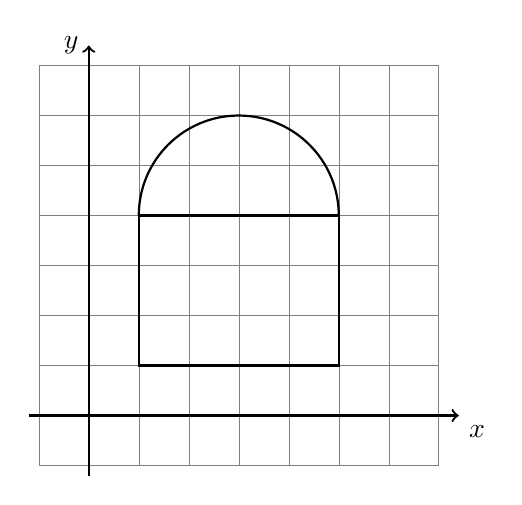
\begin{tikzpicture}[scale=.635]
  \draw [help lines] (-1,-1) grid (7,7);
  \draw [thick, ->] (-1.2,0) -- (7.4,0) node [below right] {$x$};
  \draw [thick, ->] (0,-1.2)--(0,7.4) node [left] {$y$};
  \draw [thick] (1,1)--(5,1)--(5,4)--(1,4)--cycle;
  %\draw [thick] (3,4) arc (90:270:1);
  \draw [thick] (5,4) arc (0:180:2);
\end{tikzpicture}
\end{flushright}

\item In the diagram below $\angle BOC = 7x-50$ and $\angle DOE = 4x-3$. \hfill CCSSM.8.G.B.5 \\Find $m\angle AOB$.
\vspace{0.25cm}
\begin{flushright}
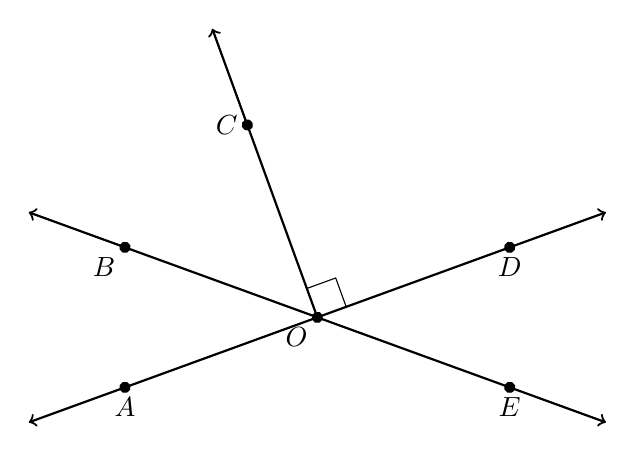
\begin{tikzpicture}[scale=1.3, rotate=20]
  \draw [<->, thick] (-40:3)--(0,0)--(140:3);
  \draw [<->, thick] (-3,0)--(3,0);
  \draw [->, thick] (0,0)--(0,3);
  \draw (0,0)++(0.3,0)--++(0,0.3)--+(-0.3,0);
  %\draw [fill] (-1,2.5) circle [radius=0.05] node[left ]{$B$};
  \draw [fill] (140:2) circle [radius=0.05] node[below left]{$B$};
  \draw [fill] (-2,0) circle [radius=0.05] node[below]{$A$}; 
  \draw [fill] (0,0) circle [radius=0.05] node[below left]{$O$};
  \draw [fill] (0,2) circle [radius=0.05] node[left]{$C$};
  \draw [fill] (2,0) circle [radius=0.05] node[below]{$D$};
  \draw [fill] (-40:2) circle [radius=0.05] node[below]{$E$};
\end{tikzpicture}
\end{flushright}


\newpage
\item A line has a gradient (slope) of $\displaystyle \frac{3}{4}$ and passes through the point $(8, 3)$. Find the equation of the line in the form $y=mx+b$.
\vspace{4cm}

\item Two lines are graphed below. 
\begin{enumerate}
  \item Complete the T-tables for each.
  \item Write down the equations for each.
\end{enumerate}
  \begin{center} 
  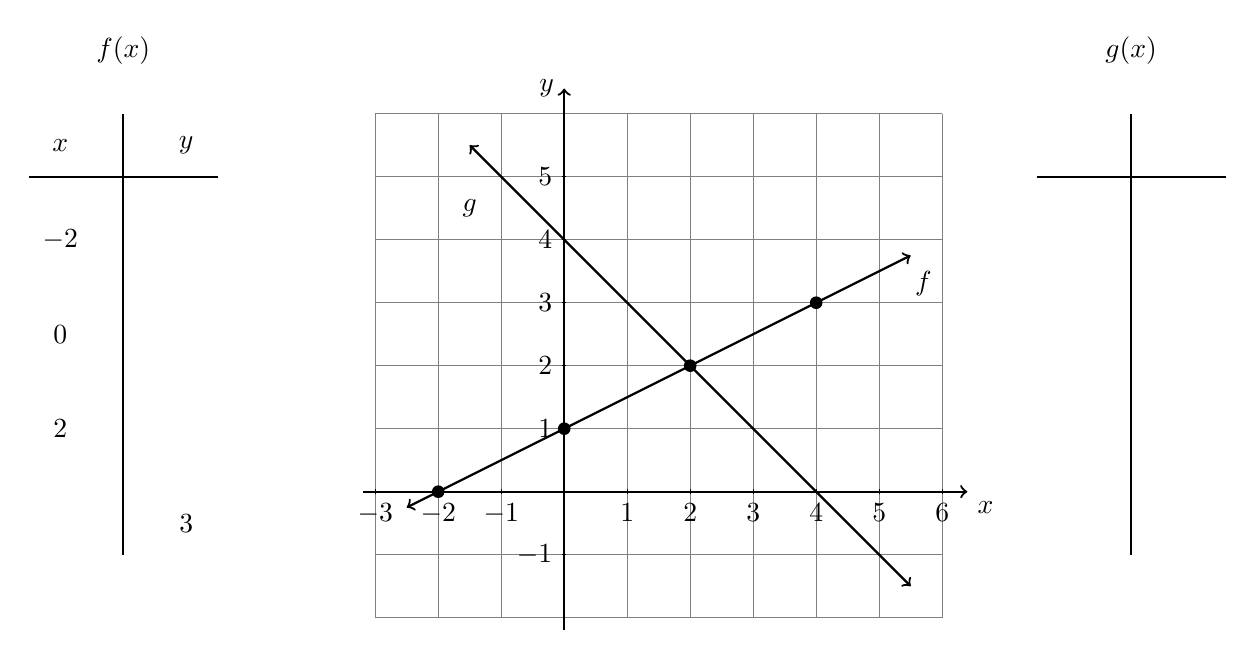
\begin{tikzpicture}[scale=0.8]
    \draw [help lines] (-3,-2) grid (6,6);
    \draw [thick, ->] (-3.2,0) -- (6.4,0) node [below right] {$x$};
    \draw [thick, ->] (0,-2.2)--(0,6.4) node [left] {$y$};
    \foreach \x in {-3,-2,-1,1,2,...,6} \draw (\x cm,1pt) -- (\x cm,-1pt) node[anchor=north] {$\x$};
    \foreach \y in {-1,1, 2, 3, 4, 5} \draw (1pt,\y cm) -- (-1pt,\y cm) node[anchor=east] {$\y$};

    \draw [thick, <->,samples=20,domain=-2.5:5.5] plot(\x,0.5*\x+1);
    \node at (5.7,3.3){$f$};
    \draw [thick, <->,samples=20,domain=-1.5:5.5] plot(\x,-1*\x+4);
    \node at (-1.5,4.5){$g$};

    \draw [thick] (-7,-1) -- (-7,6);
    \draw [thick] (-8.5,5) -- (-5.5,5);
    \node at (-7,7){$f(x)$};
    \node at (-8,5.5){$x$};
    \node at (-6,5.5){$y$};
    \draw [thick] (9,-1) -- (9,6);
    \draw [thick] (7.5,5) -- (10.5,5);
    \node at (9,7){$g(x)$};
    \node at (-8,4){$-2$}; 
    \node at (-8,2.5){$0$}; 
    \node at (-8,1){$2$}; 
    \node at (-6,-0.5){$3$};
    \fill (-2,0) circle[radius=0.1];
    \fill (0,1) circle[radius=0.1];
    \fill (2,2) circle[radius=0.1];
    \fill (4,3) circle[radius=0.1];
  \end{tikzpicture}
  \end{center}

\item A function is defined as $f(x)=2x+3$. Find each value.
\begin{enumerate}
  \begin{multicols}{2}
  \item $f(4)=$ 
  \vspace{0.5cm}
  \item $f(0)=$
  \vspace{0.5cm}
  \item $f(-3)=$
  \vspace{0.5cm}
  \item $f(1)=$
\end{multicols}\vspace{0.5cm}
  \item Find the value of $x$ that makes $f(x)=0$
\end{enumerate} \vspace{2cm}

\end{enumerate}
\end{document}